\documentclass[10pt,letterpaper]{article}
\usepackage[margin=2.1cm]{geometry}
\usepackage{fontspec}
\setmainfont{texgyretermes}[Extension=.otf,UprightFont=*-regular,BoldFont=*-bold,ItalicFont=*-italic,BoldItalicFont=*-bolditalic]
\setsansfont{texgyreheros}[Extension=.otf,Scale=0.92,UprightFont=*-regular,BoldFont=*-bold,ItalicFont=*-italic,BoldItalicFont=*-bolditalic]
\setmonofont{texgyrecursor}[Extension=.otf,Scale=0.88,UprightFont=*-regular,BoldFont=*-bold,ItalicFont=*-italic,BoldItalicFont=*-bolditalic]
\usepackage{xcolor}
\usepackage{tikz}
\usetikzlibrary{arrows.meta,positioning,fit,calc,backgrounds,shapes.callouts}
\usepackage[colorlinks=true,urlcolor=blue,citecolor=blue]{hyperref}
\usepackage{titlesec}
\titleformat{\section}{\large\bfseries}{}{0pt}{}
\titlespacing*{\section}{0pt}{0.9em}{0.3em}
\setlength{\parindent}{1.2em}
\setlength{\parskip}{0pt}
\usepackage{caption}
\captionsetup{font=small,labelfont=bf,skip=4pt}

% palette (colour-blind safe)
\definecolor{agent}{HTML}{0072B2}
\definecolor{server}{HTML}{009E73}
\definecolor{human}{HTML}{E69F00}
\definecolor{ctrl}{HTML}{7A7A7A}
\definecolor{stop}{HTML}{D55E00}

\title{\textbf{Operator-Controlled MCP:\\ A Security Layer for AI Agent Operations on Networks}}
\author{Marc Lawson\\[2pt]\small\itshape Scuola Superiore Sant'Anna, Pisa, Italy\\\small\itshape marc.lawson@santannapisa.it, monmaconair@gmail.com}
\date{}

\begin{document}
\maketitle
\thispagestyle{empty}
\vspace{-1.2em}

LLM agents are starting to get write access to real infrastructure. On a network controller one wrong call can empty a flow table, make a switch drop all its traffic, or leave a circuit half built, and none of it can be taken back. As agents begin to operate networks, the operator needs a layer between the agent and the network where what the agent does is checked, shown and approved, and a stop that does not depend on the agent choosing to stop.

We present an operator-controlled MCP~\cite{mcp} server for the Ryu OpenFlow controller~\cite{ryu}, developed in the scope of this work, as that layer. The agent can read the network freely, but every change it asks for is put under scrutiny: it is rated for risk, put to the user, approved by an operator, checked on the switch and written to a log. A person decides, and only then is anything sent. Fig.~\ref{fig:path} shows the path. The sections below list what the server offers, how we tested it and what we found. Code and tests: \href{https://github.com/maconair0/ryu-mcp-server}{\texttt{github.com/maconair0/ryu-mcp-server}}.

\begin{figure}[t]
\centering
\resizebox{\linewidth}{!}{%
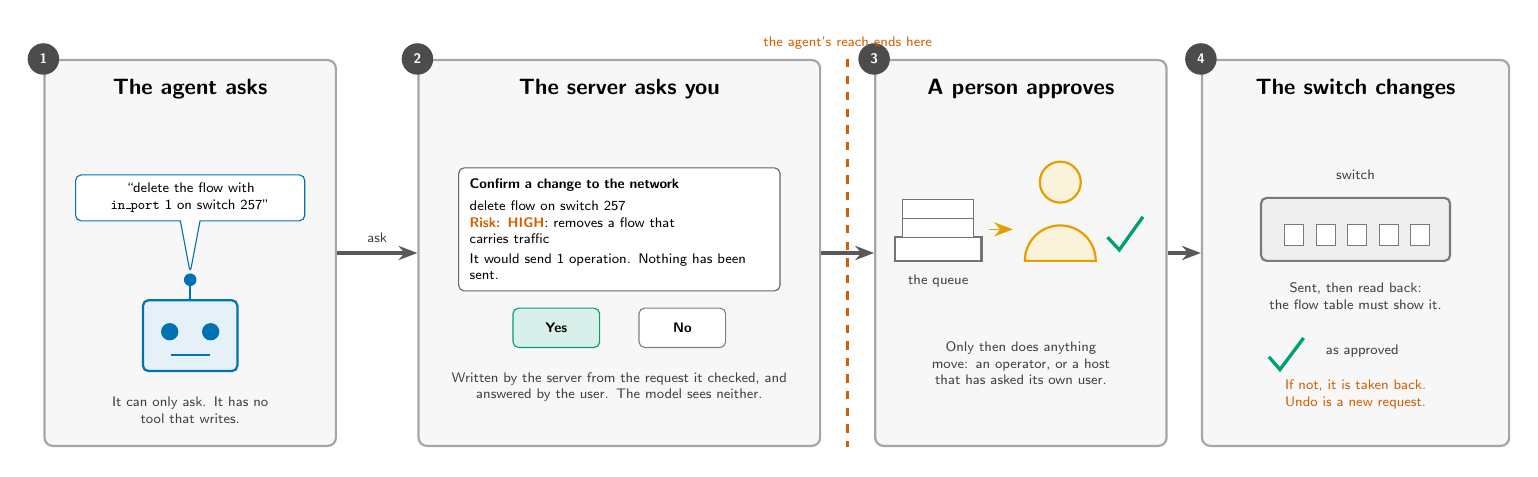
\begin{tikzpicture}[
  font=\sffamily\scriptsize,
  panel/.style={draw=black!35, rounded corners=3pt, thick, fill=black!3},
  title/.style={font=\sffamily\bfseries\footnotesize, anchor=north, inner sep=0pt},
  small/.style={font=\sffamily\tiny, text=black!75},
  arr/.style={-{Stealth[length=2.4mm]}, very thick, black!65},
  num/.style={circle, fill=black!70, text=white, font=\sffamily\bfseries\tiny, inner sep=1pt, minimum size=4mm}]
\def\h{4.9}
% ---------- panels ----------
\node[panel, minimum width=3.7cm, minimum height=\h cm] (p1) at (0,0) {};
\node[panel, minimum width=5.1cm, minimum height=\h cm] (p2) at (5.45,0) {};
\node[panel, minimum width=3.7cm, minimum height=\h cm] (p3) at (10.55,0) {};
\node[panel, minimum width=3.9cm, minimum height=\h cm] (p4) at (14.8,0) {};
\foreach \p/\t/\n in {p1/The agent asks/1, p2/The server asks you/2, p3/A person approves/3, p4/The switch changes/4} {
  \node[title] at ([yshift=-2.5mm]\p.north) {\t};
  \node[num] at (\p.north west) {\n};
}
% ---------- 1: the agent asks ----------
\begin{scope}[shift={(p1.center)}, yshift=-9mm]
  \draw[agent, thick, fill=agent!10, rounded corners=2pt] (-6mm,-6mm) rectangle (6mm,3mm);
  \fill[agent] (-2.6mm,-1mm) circle (1.1mm); \fill[agent] (2.6mm,-1mm) circle (1.1mm);
  \draw[agent, thick] (-2.5mm,-4mm) -- (2.5mm,-4mm);
  \draw[agent, thick] (0,3mm) -- (0,5mm); \fill[agent] (0,5.6mm) circle (0.8mm);
  \node[draw=agent, fill=white, rounded corners=2pt, rectangle callout, callout absolute pointer={(0,6.5mm)},
        text width=27mm, align=center, inner sep=3pt, font=\sffamily\tiny] at (0,16mm) {``delete the flow with\\ \texttt{in\_port} 1 on switch 257''};
  \node[small, text width=31mm, align=center] at (0,-11mm) {It can only ask. It has no\\tool that writes.};
\end{scope}
% ---------- 2: the server asks the user ----------
\begin{scope}[shift={(p2.center)}]
  \node[draw=black!60, fill=white, rounded corners=2pt, text width=38mm, align=left, inner sep=4pt, font=\sffamily\tiny] (card) at (0,3mm)
    {\textbf{Confirm a change to the network}\\[2pt]
     delete flow on switch 257\\
     \textbf{\textcolor{stop}{Risk: HIGH}}: removes a flow that\\carries traffic\\[1pt]
     It would send 1 operation. Nothing has been sent.};
  \node[draw=server, fill=server!15, rounded corners=2pt, minimum width=11mm, minimum height=5mm, font=\sffamily\tiny\bfseries] (yes) at (-8mm,-9.5mm) {Yes};
  \node[draw=black!50, fill=white, rounded corners=2pt, minimum width=11mm, minimum height=5mm, font=\sffamily\tiny\bfseries] (no) at (8mm,-9.5mm) {No};
  \node[small, text width=44mm, align=center] at (0,-17mm) {Written by the server from the request it checked, and\\answered by the user. The model sees neither.};
\end{scope}
% ---------- 3: a person approves ----------
\begin{scope}[shift={(p3.center)}, yshift=3mm]
  \draw[human, thick, fill=human!14] (0.5mm,-4mm) arc (180:0:4.5mm) -- cycle;
  \draw[human, thick, fill=human!14] (5mm,6mm) circle (2.6mm);
  \draw[line width=1.2pt, server] (11mm,-1mm) -- (12.5mm,-2.6mm) -- (15.5mm,1.6mm);
  % the queue: a tray of slips
  \draw[black!55, thick, fill=white] (-16mm,-4mm) rectangle (-5mm,-1mm);
  \draw[black!55, fill=white] (-15mm,-1mm) rectangle (-6mm,1.4mm);
  \draw[black!55, fill=white] (-15mm,1.4mm) rectangle (-6mm,3.8mm);
  \node[small] at (-10.5mm,-6.5mm) {the queue};
  \draw[arr, human, thin] (-4mm,0) -- (-1mm,0);
\end{scope}
\node[small, text width=33mm, align=center] at ([yshift=-14mm]p3.center) {Only then does anything\\move: an operator, or a host\\that has asked its own user.};

% ---------- 4: the switch changes, and is checked ----------
\begin{scope}[shift={(p4.center)}, yshift=1mm]
  \draw[ctrl, thick, fill=ctrl!12, rounded corners=2pt] (-12mm,-2mm) rectangle (12mm,6mm);
  \foreach \x in {-9,-5,-1,3,7} \draw[ctrl, fill=white] (\x mm,0mm) rectangle ++(2.4mm,2.6mm);
  \node[small] at (0,9mm) {switch};
  \node[small, text width=33mm, align=center] at (0,-6.5mm) {Sent, then read back:\\the flow table must show it.};
  \draw[line width=1.2pt, server] (-11mm,-14.2mm) -- (-9.6mm,-15.8mm) -- (-6.6mm,-11.8mm);
  \node[small, anchor=west] at (-5mm,-13.4mm) {as approved};
  \node[small, text width=33mm, align=center, text=stop] at (0,-19mm) {If not, it is taken back.\\Undo is a new request.};
\end{scope}
% ---------- arrows ----------
\draw[arr] (p1.east) -- (p2.west) node[midway, above, small] {ask};
\draw[arr] (p2.east) -- (p3.west);
\draw[arr] (p3.east) -- (p4.west);
% ---------- the line the agent does not cross ----------
\draw[stop, very thick, dashed] ([xshift=0mm]$(p2.north east)!0.5!(p3.north west)$ |- 0,\h/2+0.38) -- ([xshift=0mm]$(p2.south east)!0.5!(p3.south west)$ |- 0,-\h/2-0.2);
\node[small, text=stop, anchor=south, align=center] at ([xshift=0mm]$(p2.north east)!0.5!(p3.north west)$ |- 0,\h/2+0.62) {the agent's reach ends here};
\end{tikzpicture}}
\caption{The write path. The agent can only ask (1). The server puts the change to the user in its own words (2), and nothing moves until an operator decides (3). What was sent is then read back from the switch, and undone if it is not what was approved (4).}
\label{fig:path}
\end{figure}

\section*{What the server offers}

An agent can freely read the switches, links, hosts, flows and port counters, and the shortest path between two switches. Writing is where the server holds back.

\textbf{It cannot directly write:} The write tools (add or delete a flow, map or unmap a VLAN) check the request against OpenFlow's rules~\cite{of13} and put it in a queue. Nothing reaches Ryu until an operator approves it, on the command line or through a secret token that a host holds and the model never sees. No tool has a flag such as \texttt{force} or \texttt{approved} that skips the queue, because a flag the model can set is a flag the model will set.
 Each request is rated medium, high or critical, with the reasons, from what it does to the switch. A flow that drops every packet is critical, and so is deleting the flow that sends new traffic to the controller. Before a high or critical change is even queued, the server asks the person behind the client, using MCP's elicitation~\cite{elicit}. The model cannot answer for the user, because the answer is not an argument of any tool, and it cannot soften the question, because the server writes it. A no, a dismissed question or five minutes of silence queues nothing, and a critical change also needs a short code typed in. A critical change stays in the queue even when the server is set to apply changes directly.

Ryu answers 200 to flows that Open vSwitch then refuses, so the server reads the flow table back (Fig.~\ref{fig:seq}). A flow the switch does not hold is reported failed, and whatever was already sent is taken back. The flows a change replaces are read before it is sent, so an undo restores them exactly. The undo is a new request, and it waits for approval and for the user's confirmation. It is refused if a later change touched the same flows.

The approval itself is kept honest. A fingerprint of the request is checked again when it is applied, so a request edited after it was asked for is refused. A request expires after an hour, is applied once even if two processes try, and five wrong tokens in a row pause approval for five minutes. Every step, from a request to an approval, a refusal or a failure, is written to an audit log, so the operator can review what an agent asked for and what was done. If the server dies half way through a change, the next start settles it from the flow table.

\begin{figure}[t]
\centering
\resizebox{\linewidth}{!}{%
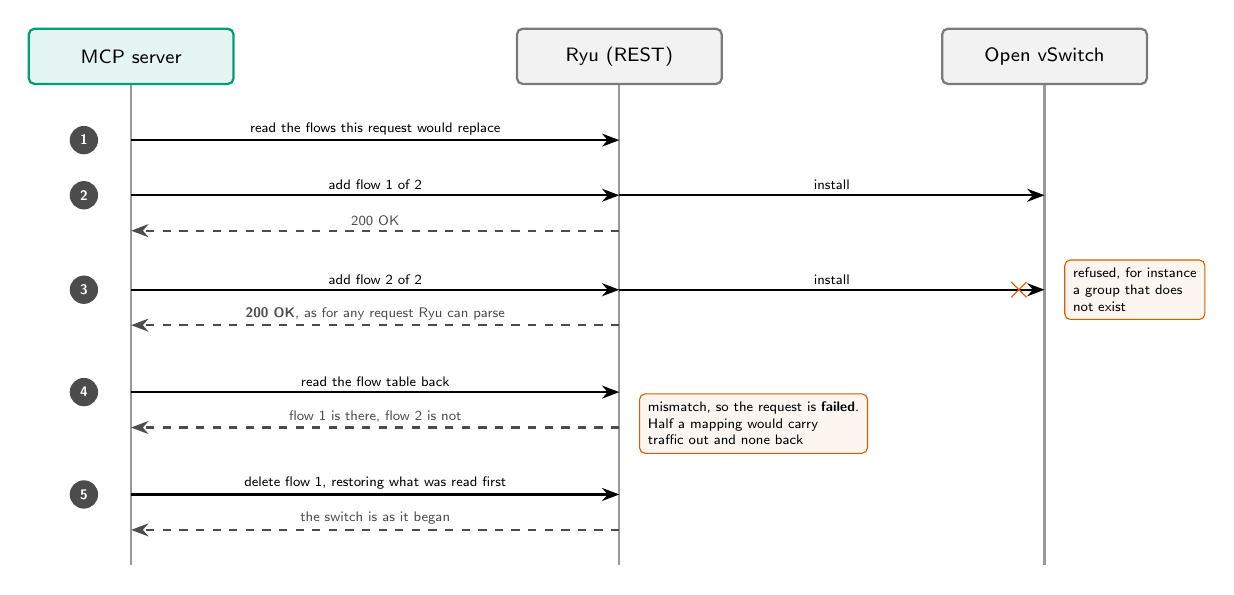
\begin{tikzpicture}[
  font=\sffamily\scriptsize,
  life/.style={thick, black!40},
  head/.style={draw, rounded corners=2pt, thick, minimum width=26mm, minimum height=7mm, inner sep=2pt, align=center},
  msg/.style={-{Stealth[length=2.2mm]}, thick},
  ret/.style={-{Stealth[length=2.2mm]}, thick, dashed, black!70},
  lab/.style={font=\sffamily\tiny, inner sep=1.5pt},
  note/.style={font=\sffamily\tiny, draw=stop, rounded corners=2pt, fill=stop!6, inner sep=3pt, align=left}]
\node[head, draw=server, fill=server!10] (S) at (0,0) {MCP server};
\node[head, draw=ctrl, fill=ctrl!10] (R) at (6.2,0) {Ryu (REST)};
\node[head, draw=ctrl, fill=ctrl!10] (W) at (11.6,0) {Open vSwitch};
\foreach \n in {S,R,W} \draw[life] (\n.south) -- ++(0,-6.1);
\newcommand{\ypos}[1]{-#1 mm}
% 1 the state before the change
\draw[msg] ([yshift=-7mm]S.south) -- ([yshift=-7mm]R.south) node[lab, midway, above] {read the flows this request would replace};
% 2 flow 1 lands
\draw[msg] ([yshift=-14mm]S.south) -- ([yshift=-14mm]R.south) node[lab, midway, above] {add flow 1 of 2};
\draw[msg] ([yshift=-14mm]R.south) -- ([yshift=-14mm]W.south) node[lab, midway, above] {install};
\draw[ret] ([yshift=-18.5mm]R.south) -- ([yshift=-18.5mm]S.south) node[lab, midway, above] {200 OK};
% 3 flow 2 is refused by the switch
\draw[msg] ([yshift=-26mm]S.south) -- ([yshift=-26mm]R.south) node[lab, midway, above] {add flow 2 of 2};
\draw[msg] ([yshift=-26mm]R.south) -- ([yshift=-26mm]W.south) node[lab, midway, above] {install};
\node[stop, font=\sffamily\bfseries\large] at ([yshift=-26mm,xshift=-3.2mm]W.south) {$\times$};
\node[note, anchor=west] at ([yshift=-26mm,xshift=2.5mm]W.south) {refused, for instance\\a group that does\\not exist};
\draw[ret] ([yshift=-30.5mm]R.south) -- ([yshift=-30.5mm]S.south) node[lab, midway, above] {\textbf{200 OK}, as for any request Ryu can parse};
% 4 read back
\draw[msg] ([yshift=-39mm]S.south) -- ([yshift=-39mm]R.south) node[lab, midway, above] {read the flow table back};
\draw[ret] ([yshift=-43.5mm]R.south) -- ([yshift=-43.5mm]S.south) node[lab, midway, above] {flow 1 is there, flow 2 is not};
\node[note, anchor=west] at ([yshift=-43mm,xshift=2.5mm]R.south) {mismatch, so the request is \textbf{failed}.\\Half a mapping would carry\\traffic out and none back};
% 5 take the part that landed back
\draw[msg] ([yshift=-52mm]S.south) -- ([yshift=-52mm]R.south) node[lab, midway, above] {delete flow 1, restoring what was read first};
\draw[ret] ([yshift=-56.5mm]R.south) -- ([yshift=-56.5mm]S.south) node[lab, midway, above] {the switch is as it began};
% step numbers on the left
\foreach \y/\n in {7/1,14/2,26/3,39/4,52/5}
  \node[circle, fill=black!70, text=white, font=\sffamily\bfseries\tiny, inner sep=1pt, minimum size=3.6mm] at ([xshift=-6mm,yshift=-\y mm]S.south) {\n};
\end{tikzpicture}}
\caption{A VLAN mapping of two flows in which the switch refuses the second. Ryu answers 200 to both, so only reading the flow table back shows it, and the flow that landed is taken back.}
\label{fig:seq}
\end{figure}

\section*{Which agents it works with}

In our setup the agent is the central agent of a multi-domain network orchestrator. It runs a 4-bit Qwen3-30B model, served locally on a single NVIDIA RTX A5000 GPU with 24~GB of memory, and it talks to the controllers only through MCP.

Nothing in the server depends on that model. It speaks the standard Model Context Protocol, over SSE or over standard input and output, so any MCP client can use it, including agents built on hosted models such as Claude or GPT. Connecting one takes the address of the server, or the command that starts it (\texttt{run\_ryu\_mcp.py}), and nothing else. The safeguards live in the server and not in the model, which is what makes it a security layer for any agent and not a feature of one: a hosted model meets the same queue, the same ratings and the same approval as our local one. The user's confirmation needs a client that implements elicitation. A client that does not can still use the server, and then the operator's approval alone stands, or the write is refused if the server runs strict. We tried only the local model in the chat tests, and the tests on the server itself used scripted and random callers, so hosted models are untested.

\section*{How we tested it, and what we found}

We tried to break the server in four ways: unit tests against a fake of Ryu's REST API that behaves like a live one, 15 scripted attacks plus a fuzzer of 25,000 random calls, mutation testing that switches each guard off in turn, and a stress run on a live lab Ryu with three Open vSwitch switches, which ended by undoing every change and comparing the flow tables with the start.

No write reached a switch without a decision, in the attacks or the fuzzing, and every approved request was applied. The attacks included arguments that look like consent, a wildcard drop-all, a burst of 300 requests, a queue entry rewritten after it was asked for, and 100 kB token guesses. On the live Ryu, 64 callers made 638 reads with no errors, and a flood of 320 write requests queued exactly the hourly cap of 20. Twenty requests approved at once from two paths were each applied exactly once, and undoing all of them restored the 34 flows exactly.

The tests found more about our own code than the attacks did. The first mutation run missed four of 17 guards, and all 29 are now caught. A live controller showed what the fake had hidden: four requests that Ryu accepted never reached the switch, and an action written in lower case installed a flow with no actions, which drops traffic. A process killed in the middle of a change left it claimed forever, which is why the server now recovers it. These are fixed and covered by tests.

\section*{What it does not cover}

No language model tried to outwit the standalone server, and the user's confirmation was tested with test clients and not a production agent host. Approval is only as good as the person approving, and whoever can write the server's state directory is in effect the operator. An undo is exact only for what can be read back. Read-back shows the switch holds the flow, not that traffic does what the person wanted. The scope is OpenFlow 1.3 through one version of Ryu.

\section*{Conclusion}

The server is a security layer between AI agents and the network. It leaves reading open, and puts every change under the scrutiny of an operator and of the user: rated, put to the user in the server's own words, approved, checked on the switch and written to an audit log. An agent that can only ask cannot make an irreversible change on its own. Nothing reached a switch without a decision in any test, and every change made to a live network was taken back exactly.

\begin{thebibliography}{9}\footnotesize\setlength{\itemsep}{0pt}
\bibitem{mcp} Anthropic, Model Context Protocol (2024).
\bibitem{ryu} Ryu SDN Framework, \texttt{ryu-sdn.org}.
\bibitem{of13} Open Networking Foundation, OpenFlow Switch Specification, v1.3.
\bibitem{elicit} Model Context Protocol, Specification: Elicitation (2025).
\end{thebibliography}
\end{document}
